\documentclass{article}

\usepackage[pdftex]{geometry}	% Use A4 paper margins
\usepackage[english]{babel}
\usepackage{graphicx}
\usepackage{url}
\usepackage{hyperref}
\usepackage{float}
\usepackage{xcolor} % Required for specifying custom colors
\usepackage{fix-cm} % Allows increasing the font size of specific fonts beyond LaTeX default specifications
\usepackage{tikz}
\usepackage{listings}
\usepackage{pgfplots}
\usepackage{float}
\usepackage{todonotes}
\usepackage{rotating}
\usepackage{pgfplotstable}

\setlength{\oddsidemargin}{0mm} % Adjust margins to center the colored title box
\setlength{\evensidemargin}{0mm} % Margins on even pages - only necessary if adding more content to this template

\newcommand{\HRule}[1]{\hfill \rule{0.2\linewidth}{#1}} % Horizontal rule at the bottom of the page, adjust width here
\renewcommand{\familydefault}{\sfdefault}

\graphicspath{{./images/}}

\begin{document}

\begin{titlepage}

  {\Huge ATX PSU Dev Board }\\
  {\Large Assembly Instructions for v0.1} 
  \vspace*{\fill}	
  \begin{center}
  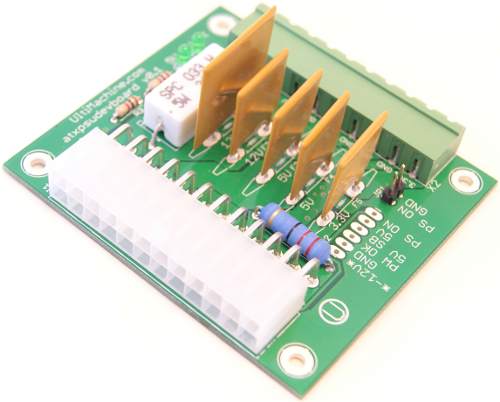
\includegraphics[scale=0.75]{png/ATX_PSU_Dev_PreAssembled2.png}
  \end{center}
  \vspace*{\fill}

  \vfill
  {\centering \large 
  \hfill 
\includegraphics[scale=0.75]{png/um_logo.png} \\
  \hfill \url{http://ultimachine.com/content/atx-psu-dev-board} \\

  \HRule{1pt}} % Horizontal line, thickness changed here
\end{titlepage}

\clearpage % Whitespace to the end of the page

\tableofcontents
\clearpage

\section{Overview}

\subsection{Introduction}

\subsubsection{What's in the box}

\begin{figure}[htbp]
\centering
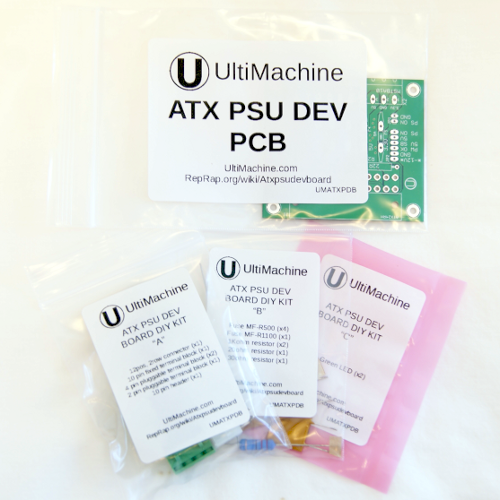
\includegraphics{./png/kit.png}
\caption{Bag Layout}
\end{figure}

\subsection{Assembly}

\subsubsection{Preparation}

\paragraph{Tools}

The following tools and materials are required to assemble the ATX PSU
Dev Board:

\begin{itemize}
\item
  Soldering Iron
\item
  Solder
\item
  Flush/diagonal cutters
\end{itemize}

Additional tools that might be helpful, but not required:

\begin{itemize}
\item
  Lead bender
\end{itemize}

\paragraph{Soldering}

If you do not have prior experience soldering, we recommend checking out
a few of the following websites for some tutorials.

\begin{itemize}
\item
  \url{http://mightyohm.com/files/soldercomic/FullSolderComic_EN.pdf}
\item
  \url{http://www.ladyada.net/media/common/soldering.pdf}
\item
  \url{http://store.curiousinventor.com/guides/How_to_Solder}
\item
  \url{http://www.sparkfun.com/tutorials/106}
\item
  \url{http://radiojove.gsfc.nasa.gov/telescope/soldering.htm}
\end{itemize}

\subsubsection{Assembly}

The components of this board will be inserted on the side with the
outlines

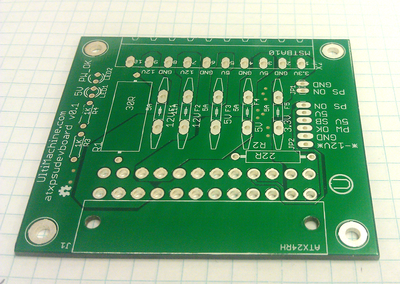
\includegraphics{./png/correct-side.png}
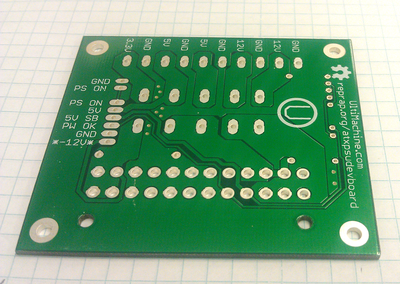
\includegraphics{./png/incorrect-side.png}

Begin by inserting the two 1k ohm resistors and the LEDs into the board.
The LEDs should have the longest lead in the hole facing the resistor.
If they are inserted incorrectly they will not work. This is because
they are diodes. Resistors are not polarized components, so they can be
inserted in orientation.

\begin{figure}[htbp]
\centering
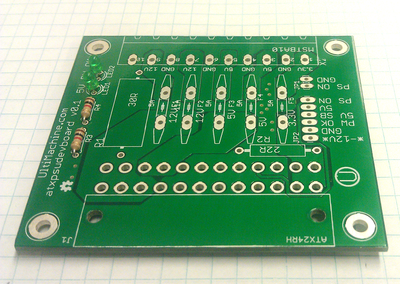
\includegraphics{./png/step-01.png}
\caption{Step 1}
\end{figure}

Next flip over the board and solder the components in.

\begin{figure}[htbp]
\centering
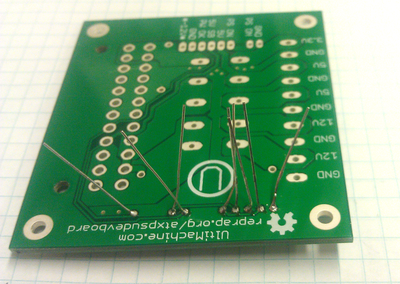
\includegraphics{./png/step-02.png}
\caption{Step 2}
\end{figure}

Now that the components are soldered in and secure you can cut the
leads.

\begin{figure}[htbp]
\centering
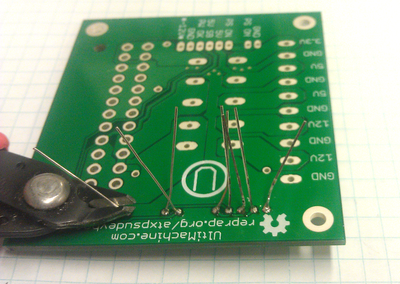
\includegraphics{./png/step-03.png}
\caption{Step 3}
\end{figure}

The fuses will be inserted next. They have a coating that slightly
descends down the leads.

\begin{figure}[htbp]
\centering
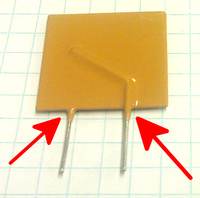
\includegraphics{./png/fuse.png}
\caption{Resetable Fuse}
\end{figure}

In order to make a good connection the fuses should slightly hover over
the holes. This is so the coating on the leads does not interfere with
soldering. You want to bring the fuse above the board. You can do this
with RepRap filament or something else, such as a long screw. The
orientation of the fuses does not matter.

\begin{figure}[htbp]
\centering
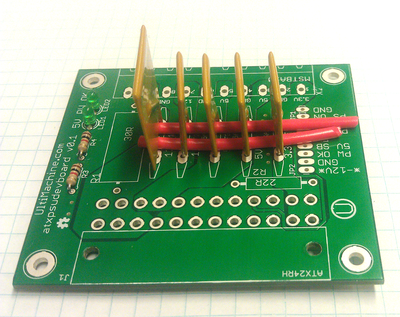
\includegraphics{./png/step-04.png}
\caption{Step 4}
\end{figure}

You can remove the filament.

\begin{figure}[htbp]
\centering
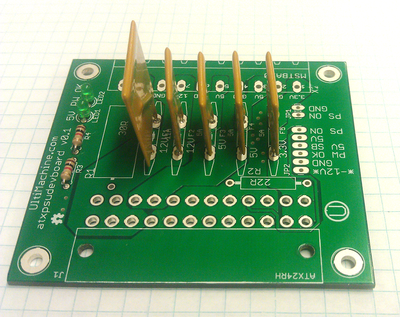
\includegraphics{./png/step-05.png}
\caption{Step 5}
\end{figure}

Now is a good opportunity to check that all connections were soldered
well. Ideally the solder should wick up the lead onto the other side of
the board. It should also have a nice tapered look. Add some flux and
reheat the joint to touch-up the connections if needed. \textbackslash{}

Now is a good opportunity to inspect the solder joints. Since the
connectors and fuses on this board might carry a good amount of current
you want a good solder flow. You can check the quality of the solder
joint by looking at the other side of the leads. A good connection is
shown on the left lead, with a potentially weak one on the right lead.

\begin{figure}[htbp]
\centering
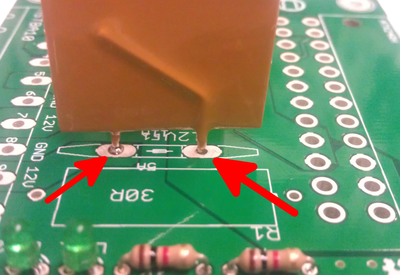
\includegraphics{./png/solder-joint.png}
\caption{Solder Joint}
\end{figure}

Next you will want to solder in the remaining resistors. Again,
orientation does not matter for resistors.

\begin{figure}[htbp]
\centering
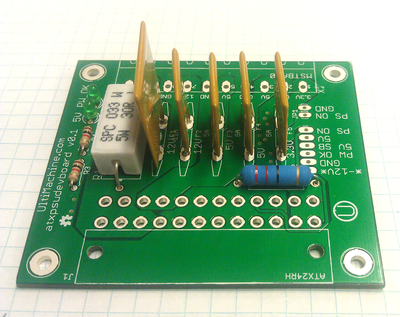
\includegraphics{./png/step-06.png}
\caption{Step 6}
\end{figure}

Next locate the header pins in the parts bag. You will need to break
them into a strip of 6 and 2 as shown below. This can be done with flush
cutters.

\begin{figure}[htbp]
\centering
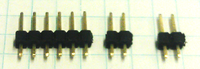
\includegraphics{./png/header-break.png}
\caption{Split header pins}
\end{figure}

Solder the header pins as shown.

\begin{figure}[htbp]
\centering
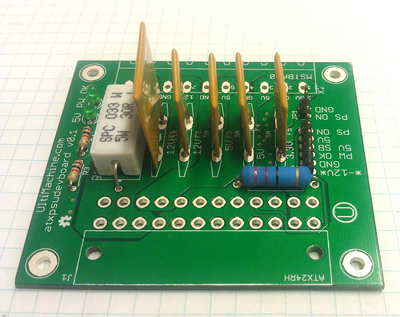
\includegraphics{./png/step-07.png}
\caption{Step 7}
\end{figure}

Add the recieving end for the pluggable headers.

\begin{figure}[htbp]
\centering
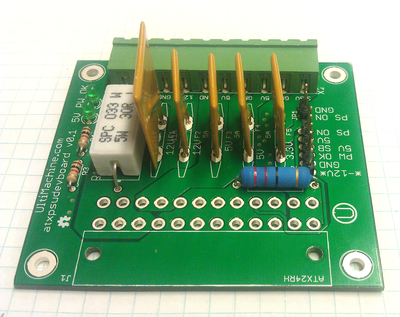
\includegraphics{./png/step-08.png}
\caption{Step 8}
\end{figure}

Next you will want to add the ATX connector. It has barbs on the housing
that should clip onto the circuit board. Make sure the connector is well
seated before soldering.

\begin{figure}[htbp]
\centering
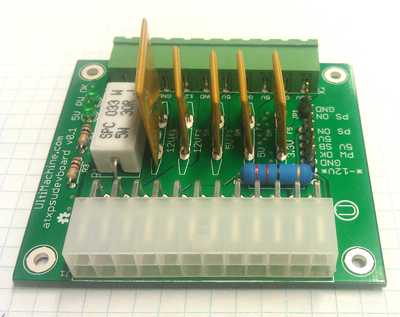
\includegraphics{./png/step-09.png}
\caption{Step 9}
\end{figure}

You have now completed assembly of the ATX PSU Dev Board!

\section{Usage}

\begin{figure}[htbp]
\centering
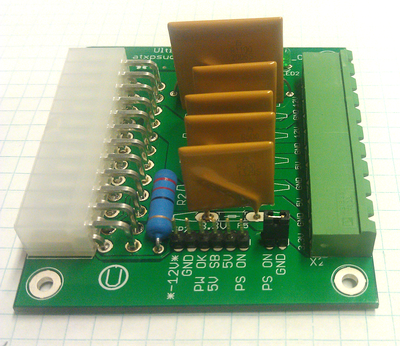
\includegraphics{./png/step-10.png}
\caption{PS\_ON Jumper}
\end{figure}

\begin{figure}[htbp]
\centering
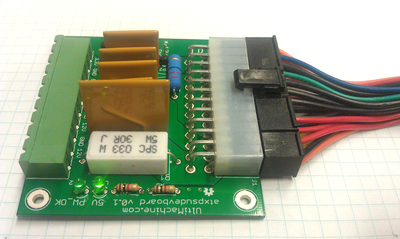
\includegraphics{./png/step-11.png}
\caption{Testing a power supply}
\end{figure}

\begin{figure}[htbp]
\centering
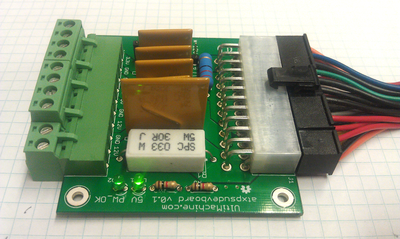
\includegraphics{./png/step-12.png}
\caption{Pluggable headers inserted}
\end{figure}

\section{Source}


\end{document}
